\section{CapFill: Capacitance Estimation and Native Integration}
CapFill first encodes the observed response and the geometry to be evaluated. A support-based anchor and a learned residual share the same output scales, so each numerical or neural candidate can contribute a correction in the same units. The estimator fuses the applicable corrections, restores physical units, and passes the resulting values to the selected preparation interface.

\subsection{Input Encoding and Contextual Representation}
Each geometry has three coordinates (width and two spacings) and a context vector $\mathbf c$ with four family indicators, three layer indices divided by 16, three material features and a material-availability flag. Each geometry token has $17+2K$ features. For source scales $\mathbf s_x,\mathbf s_y$, observation indicator $o_i$, and physical-unit anchor $\mathbf b^{\rm phys}_i$, define
\begin{align}
\widetilde{\mathbf x}_i&=\log(1+\mathbf x_i\oslash\mathbf s_x),&
\widetilde{\mathbf y}_i&=\mathbf y_i^{\rm in}\oslash\mathbf s_y,\\
\mathbf b_i&=\mathbf b_i^{\rm phys}\oslash\mathbf s_y,&
\mathbf f_i&=[\widetilde{\mathbf x}_i;\mathbf c;\widetilde{\mathbf y}_i;o_i;\mathbf b_i;1;0].
\end{align}
The input $\mathbf y_i^{\rm in}$ contains the supplied response when $o_i=1$ and a zero vector otherwise. The indicator distinguishes a withheld response from an observed zero. Coordinate scales are source median absolute coordinates (one for a zero median). Component scales are family-specific source RMS values floored at $10^{-3}$ of pooled RMS. Geometry tokens retain the supplied coordinate order. Appended material tokens encode layer bottom, top and relative permittivity on logarithmic scales, copy context, zero-fill response channels, and use type bits $[0,1]$.

A two-layer, four-head Transformer of width 64 processes the projected features $\mathbf F$ with a padding mask $M$:
\begin{equation}
\mathbf H^0=\mathbf F W_{\rm in}+b_{\rm in},\quad
\mathbf H^2=\operatorname{Enc}_\theta(\mathbf H^0,M),\quad
\mathbf h_i=\mathbf H^2_i\in\mathbb R^{64}.
\end{equation}
Each pre-normalized encoder layer has a 256-unit feedforward block. Padding tokens are excluded as attention keys. The residual and gate use the same query representation. Because queries attend to each other, batch composition affects predictions. The native preparation protocol therefore fixes query ordering and chunk size.

\subsection{Numerical Anchor and Correction Basis}
For interpolation, each coordinate is centered at its observed minimum and scaled by its observed range (one for a constant axis). After merging equal coordinates with equal values, we retain axes in order whenever they increase affine rank at tolerance $10^{-10}$. Conflicting duplicate labels are rejected. Rank zero gives a constant anchor. At rank one we interpolate linearly and clamp to the observed endpoints. At higher rank we use barycentric interpolation on the Delaunay simplex of the projected query. Outside that triangulation, or on triangulation failure, we use the nearest observation in reduced coordinates. Equal distances select the first lexicographically sorted unique coordinate. Exact observations are restored.

Full uses eleven slots $\mathcal E$: Anchor, PCHIP, WidthLinear, six RBF-GPs, NN and NN-Clip. Each estimates a correction $\Delta_{i,e,k}=f_{i,e,k}-b_{i,k}$ in source-normalized units for component $k$. Anchor always supplies zero correction. On single-width curves, PCHIP evaluates the shape-preserving cubic Hermite interpolant of ordered observed knots at the clamped query. Between knots $t_0,t_1$, the cubic matches the observed values and the monotonicity-preserving endpoint derivatives. At an interior knot, derivatives vanish at a secant sign change and otherwise use a weighted harmonic mean. WidthLinear requires equal non-width coordinates and either an exact width or two bracketing observed widths. Its upper-width weight is $(w-w_-)/(w_+-w_-)$. Each GP uses the centered observed outputs and kernel
\begin{equation}
\begin{aligned}G_{ab}&=\exp[-\|\mathbf z_a-\mathbf z_b\|^2/(2\ell^2)],\\
f(q)&=\bar y+G_{qS}(G_{SS}+\lambda I)^{-1}(y_S-\bar y).\end{aligned}
\end{equation}
Here $\mathbf z$ denotes reduced coordinates. The length scale is the median positive observed pair distance times $0.5$, 1 or 2, with ridge $\lambda=10^{-6}$ or $10^{-4}$. Each GP restores exact observations and clips negative estimates to zero. A classical branch is valid only where applicable and finite in all components.

\subsection{Observation-Conditioned Residual Gating}
The neural head predicts $\boldsymbol\delta_i=W_r\mathbf h_i+b_r$. NN uses this residual directly. NN-Clip limits the completed value to the component-wise extrema $L_i,U_i$ of the bracketing knots or simplex vertices:
\begin{equation}
\Delta_{i,\mathrm{clip}}=
\begin{cases}
\operatorname{clip}(\mathbf b_i+\boldsymbol\delta_i,L_i,U_i)-\mathbf b_i,&\mathbf x_i\in\Omega,\\
\boldsymbol\delta_i,&\text{otherwise}.
\end{cases}
\end{equation}
Here $\mathbf x_i\in\Omega$ requires both full-space affine membership (maximum normalized reconstruction residual $\le10^{-9}$) and projected interval or simplex membership. This test distinguishes an off-plane query from one inside the hull with the same projected coordinates.

Let $m_{i,e}$ indicate branch validity, let $\mathcal E_i=\{e:m_{i,e}=1\}$ contain the valid candidates, $N_i=|\mathcal E_i|$, and write $\langle d\rangle_i=N_i^{-1}\sum_{e\in\mathcal E_i}d_e$. For each component the gate computes
\begin{align}
\mu_{ik}&=\langle\Delta_{i,e,k}\rangle_i,\\
\sigma_{ik}&=\sqrt{\langle(\Delta_{i,e,k}-\mu_{ik})^2\rangle_i+10^{-12}},\\
r_{ik}&=\max_{e\in\mathcal E_i}\Delta_{i,e,k}-\min_{e\in\mathcal E_i}\Delta_{i,e,k}.
\end{align}
The descriptor $\mathbf u_i$ includes observed fraction, nearest-support distance, local vertex span, scaled envelope width, inside flag, affine rank, typical neighbor distance and width validity. Five indicators distinguish outside, missing interior width, dense rank-one, dense higher-rank and sparse/degenerate support. Further features give per-axis fractions of observations below the query, local variation, slope and slope change from up to three nearest observations, and context $\mathbf c$.
\ifdefined\CapFillExtendedThe support fraction divides distinct observed coordinates by the number of candidate coordinates in the current table. The distance features use all support-range-normalized coordinates. Local span is the Euclidean norm of the coordinate ranges of the enclosing vertices, zero outside. Envelope width is divided component-wise by the source response scale. Distance, span and envelope width use $\log(1+z)$. Typical spacing is the median nearest-neighbor distance among distinct observations. A positive typical spacing and a local span at most twice that spacing identify dense support. Outside membership takes precedence, followed by an unobserved width strictly between the minimum and maximum observed widths, then the dense rank-one and higher-rank cases.

For variation and slopes, order the three nearest observations by distance with stable input-order ties. Variation is the component range of their scaled responses. The first slope divides the second-minus-first response by the distance between those observations, floored at $10^{-12}$. Curvature subtracts that slope from the corresponding second-to-third slope. Unavailable derivatives are zero. The gate receives log typical spacing and variation, signed-log slopes and curvature, and the same context as the geometry tokens. Material tokens occupy the same feature width as geometry tokens, $17+2K$.
\fi

With $\phi(z)=\operatorname{sign}(z)\log(1+|z|)$ the gate forms
\begin{align}
v_i&=[\mathbf h_i;\mathbf u_i;\phi(\mu_i);\phi(\sigma_i);\phi(r_i)],\\
a_i&=W_2\operatorname{ReLU}(W_1v_i+b_1)+b_2,\\
\pi_{i,e,k}&=\frac{\exp((a_{i,e,k}+\beta_e)/\tau)}
{\sum_{j\in\mathcal E_i}\exp((a_{i,j,k}+\beta_j)/\tau)},\quad e\in\mathcal E_i,\\
\widehat y_{i,k}&=s_{y,k}\left[b_{i,k}+
\sum_{e\in\mathcal E_i}\pi_{i,e,k}\Delta_{i,e,k}\right]_+ .
\end{align}
The hidden gate width is 32. The implementation emits $11\times K$ logits, giving $a_i|_{\mathcal E_i}\in\mathbb R^{N_i\times K}$ after restriction. Invalid logits are masked at $-10^9$ before softmax. Both neural slots are valid, with nonfinite corrections set to zero. Initial prior offsets are zero for Anchor and the neural branches and $-8$ (public) or $-2$ (FEM and transfer) for the other branches. The learned temperature $\tau=\operatorname{softplus}(\theta_\tau)+0.001$ starts at 0.251. Projection $[z]_+=\max(0,z)$ precedes conversion to physical units. Binary gates only Anchor and NN from context and support descriptors, omitting candidate-agreement features. Ungated adds NN directly.

\subsection{Training Objective}
Each source episode partitions a table into observed support and withheld queries. Sampling balances pattern families and selects a process and table within family. Across the three variants, the source pools, residual initialization, masks and update budgets are matched. The Huber loss with unit threshold averages component errors $(\widehat y_{i,k}-y_{i,k})/s_{y,k}$ over withheld queries. Thus the residual branch receives supervision through the completed estimate. At inference only observed labels are supplied.

\subsection{Native Compute-Table Population}
OpenRCX first constructs its distance table from a process/corner rule (Fig.~\ref{fig:interface}). A slot key identifies the rule, family, layers, mapped width, slot index, represented separation, components and units. Eligible slots $\mathcal J$ require a unique source match, at least four matched observations, and a finite interior location in OVER, UNDER or OVERUNDER. Measurement-bin collisions, sentinels, special tails, unsupported paths and resistance are excluded. The coordinates presented to the model are those represented by the native slots.

\begin{figure*}[t]\centering
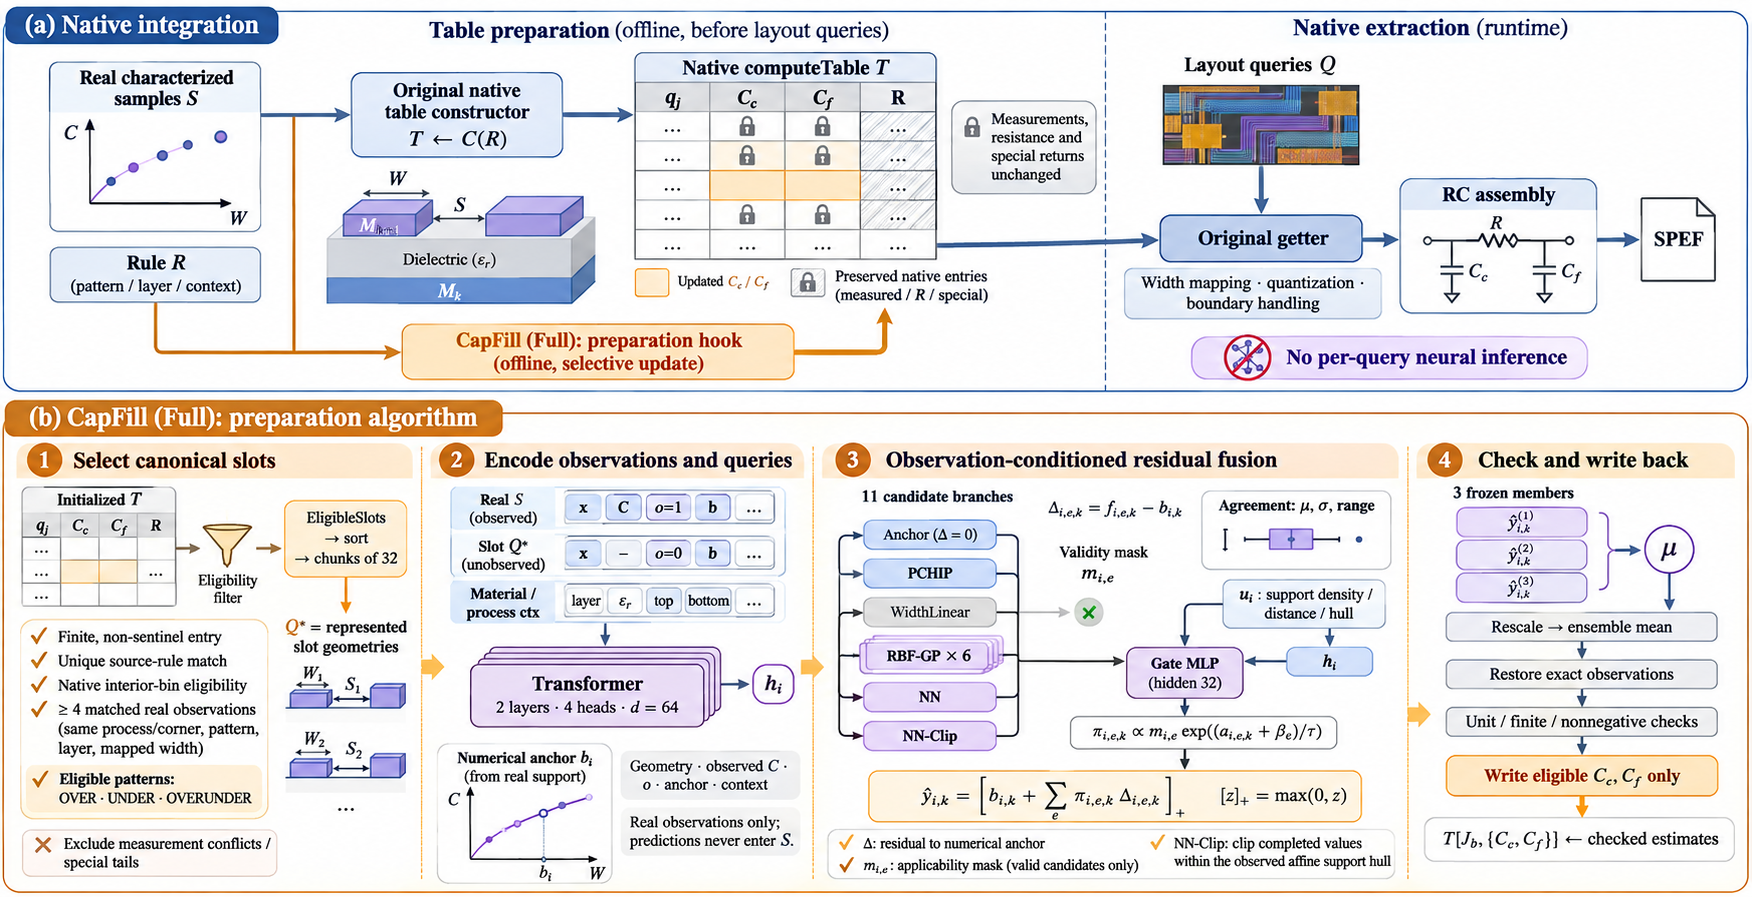
\includegraphics[width=\textwidth]{figures/compute_table_interface.png}
\caption{CapFill prepares coupling and fringe entries after native compute-table construction. During extraction, the native getter maps layout geometry to a width and distance bin and supplies capacitances for RC assembly.}\label{fig:interface}
\end{figure*}
\begin{algorithm}[t]
\caption{Prepare eligible native compute-table entries}\label{alg:prepare}
\Input{Rule $\mathcal R$, characterized support $S$, three frozen Full members}
\Output{Prepared native table $T$}
$T\gets\operatorname{NativeConstruct}(\mathcal R)$\;
$\mathcal J\gets\operatorname{EligibleSlots}(T,\mathcal R,S)$\;
Sort within each rule context by separation, then complete slot key\;
\ForEach{successive chunk $J_b\subseteq\mathcal J$ of at most 32 slots}{
  Assemble unique support coordinates then unseen query coordinates\;
  Retain slot-to-token indices and append material tokens\;
  \ForEach{frozen member $m$}{
    Encode $S,Q_b,c$ and evaluate valid corrections and gates\;
    Project to nonnegative values and rescale to physical units\;
    Gather $\widehat Y_b^{(m)}$ using slot-to-token indices\;
  }
  $Y_b\gets\operatorname{RestoreExact}(S,Q_b,\frac13\sum_m\widehat Y_b^{(m)})$\;
  Convert units and check finiteness and nonnegativity\;
  Write $Y_b$ to coupling ($C_c$) and fringe ($C_f$) fields of $T[J_b]$\;
}
\Return{$T$}\;
\end{algorithm}
Algorithm~\ref{alg:prepare} reuses the characterized support across chunks. Generated values never become observations. Original measurement returns and special paths remain available to the getter. The release executable retains native width selection, quantization and RC assembly, while a separate trace build checks returned values.
